\normalfont\documentclass[letterpaper,11pt]{article}
\usepackage{amsmath, amsfonts,amssymb,latexsym}
\usepackage{fullpage}
\usepackage{parskip}
\usepackage{flexisym}
\usepackage{indentfirst}
\usepackage{graphicx}
\usepackage{algorithm2e}
% \usepackage{algorithm}
\usepackage{algorithmicx}
% \usepackage{algpseudocode}
\usepackage{amsmath}
\begin{document}
\setlength{\parindent}{2ex}
\newcommand{\header}{
	\noindent \fbox{
	\begin{minipage}{6.4in}
	\medskip
	\textbf{CS 271 -  Introduction to Artificial Intelligence} \hfill \textbf{Fall 2016} \\[1mm]
	\begin{center}
		{\Large HomeWork 6} \\[3mm]
	\end{center}
	  Name: \itshape{Liangjian Chen} \\
	  \textnormal{ID}: \itshape{\#52006933} \hfill \today
	\medskip
	\end{minipage}}
}
\bigskip
\header

\begin{enumerate}
\item[Problem 1]\textbf{Solution:}\par
	\begin{enumerate}
		\item \par
			In original expression, $x$ and $y$ could be same. Thus it should be revised as following:
			$$\neg \exists x,y,n\text{ }Person(x) \land Person(y) \land \neg(x = y) \land HasSS\#(x,n) \land HasSS\#(y,n)$$ 
		\item \par
			Yes, it is correct.
		\item \par
			No. In original expression, it said that everyone has every different SSN, which obviously incorrect.
			$$\forall x,n\text{ }Person(x) \land HasSS\#(x,n) \Rightarrow Digits(n,9)$$
		\item \par
		Assume $SS\#(x)$ means $x$'s social security number.
		$$\neg \exists x,y\text{ }Person(x) \land Person(y) \land (SS\#(x) = SS\#(y))$$
		$$SS\#(John) = SS\#(Mary)$$
		$$\forall x\text{ }Person(x) \Rightarrow Digits(SS\#(x),9)$$
	\end{enumerate}
\item[Problem 2]\textbf{Solution:}\par
	\begin{enumerate}
		\item No
		\item $x = A, y = B , z = B$
		\item $x = David, father(x) = George$
		\item $x = g(u) = g(f(v))$
		\item $x = y = z = B$
	\end{enumerate}
\item[Problem 3]\textbf{Solution:}\par
	$Alpine(x)$ means $x$ is in the Alpine club. $skier(x)$ means $x$ is skier, $climber(x)$ means $x$ is climber. $Like(a,b)$ means $a$ likes $b$.
	\begin{align*}
		&Alpine(Tony), Alpine(Mike), Alpine(John).\\
		&\forall x, Alpine(x)  \Rightarrow skier(x)\lor climber(x)\\
		&\forall x, climber(x) \Rightarrow \neg like(x,Rain) \\
		&\forall x, skier(x) \Rightarrow like(x,snow) \\
		&\forall x, like(John, x) \Rightarrow \neg like(Mike, x)\\
		&\forall x, \neg like(John, x) \Rightarrow like(Mike, x)\\
		&\neg like(John, rain)\\
		&\neg like(John, snow)
	\end{align*}
	Then, question is
	$\exists x,Alpine(x) \land climber(x) \land \neg skier(x)$.\\
	By negating the answer term, we obtain $\forall x,\neg Alpine(x) \lor \neg climber(x) \lor skier(x)$.\\
	Convert the original expression to CNF form plus the answer term we obtain.
	\begin{align}
		&Alpine(Tony), Alpine(Mike), Alpine(John).\\
		&\neg Alpine(x_1)  \lor skier(x_1)\lor climber(x_1)\\
		&\neg climber(x_2) \lor \neg like(x_2,Rain) \\
		&\neg skier(x_3) \lor like(x_3,snow) \\
		&\neg like(John, x_4) \lor \neg like(Mike, x_4)\\
		&like(John, x_5) \lor \neg like(Mike, x_5)\\
		&\neg like(John, rain)\\
		&\neg like(John, snow)\\
		&\neg Alpine(x_6) \lor \neg climber(x_6) \lor skier(x_6)\\
		&\neg skier(John) \lor like(John,snow)\{4,x_3/John\} \\
		&\neg skier(John)\{8,10\}\\
		& climber(John)\{1,2,11\}\\
		& Alpine(John) \land climber(John) \land \neg siker(John)\{1,11,12\}\\
		&\neg Alpine(John) \lor \neg climber(John) \lor skier(John)\{9,x_6/John\}\\
		&Empty\{13,14\}
	\end{align}
	substitute $x_6$ by $John$, we can find it contradict with (13), and it show John is the answer.
\item[Problem 4]\textbf{Solution:}\par
	\begin{enumerate}
		\item Yes.
		\item No.
		\item No.
	\end{enumerate}
\item[Problem 5]\textbf{Solution:}\par
	\begin{enumerate}
		\item 
		$$\forall x, Horse(x) \Rightarrow mammals(x)$$
		$$\forall x, Cow(x) \Rightarrow mammals(x)$$
		$$\forall x, Sheep(x) \Rightarrow mammals(x)$$
		\item 
		$$\forall x,y, Pig(y) \land offspring(x,y) \Rightarrow Pig(x)$$
		\item 
		$$Pig(Bluebeard)$$
		\item
		$$parent(Bluebeard,Charlies)$$
		\item
		$$\forall x,y, parent(x,y) \Leftrightarrow offspring(y,x)$$
		\item
		$$\forall x,mammals(x) \Rightarrow \exists y, parent(y,x)$$
	\end{enumerate}	
\item[Problem 6]\textbf{Solution:}\par
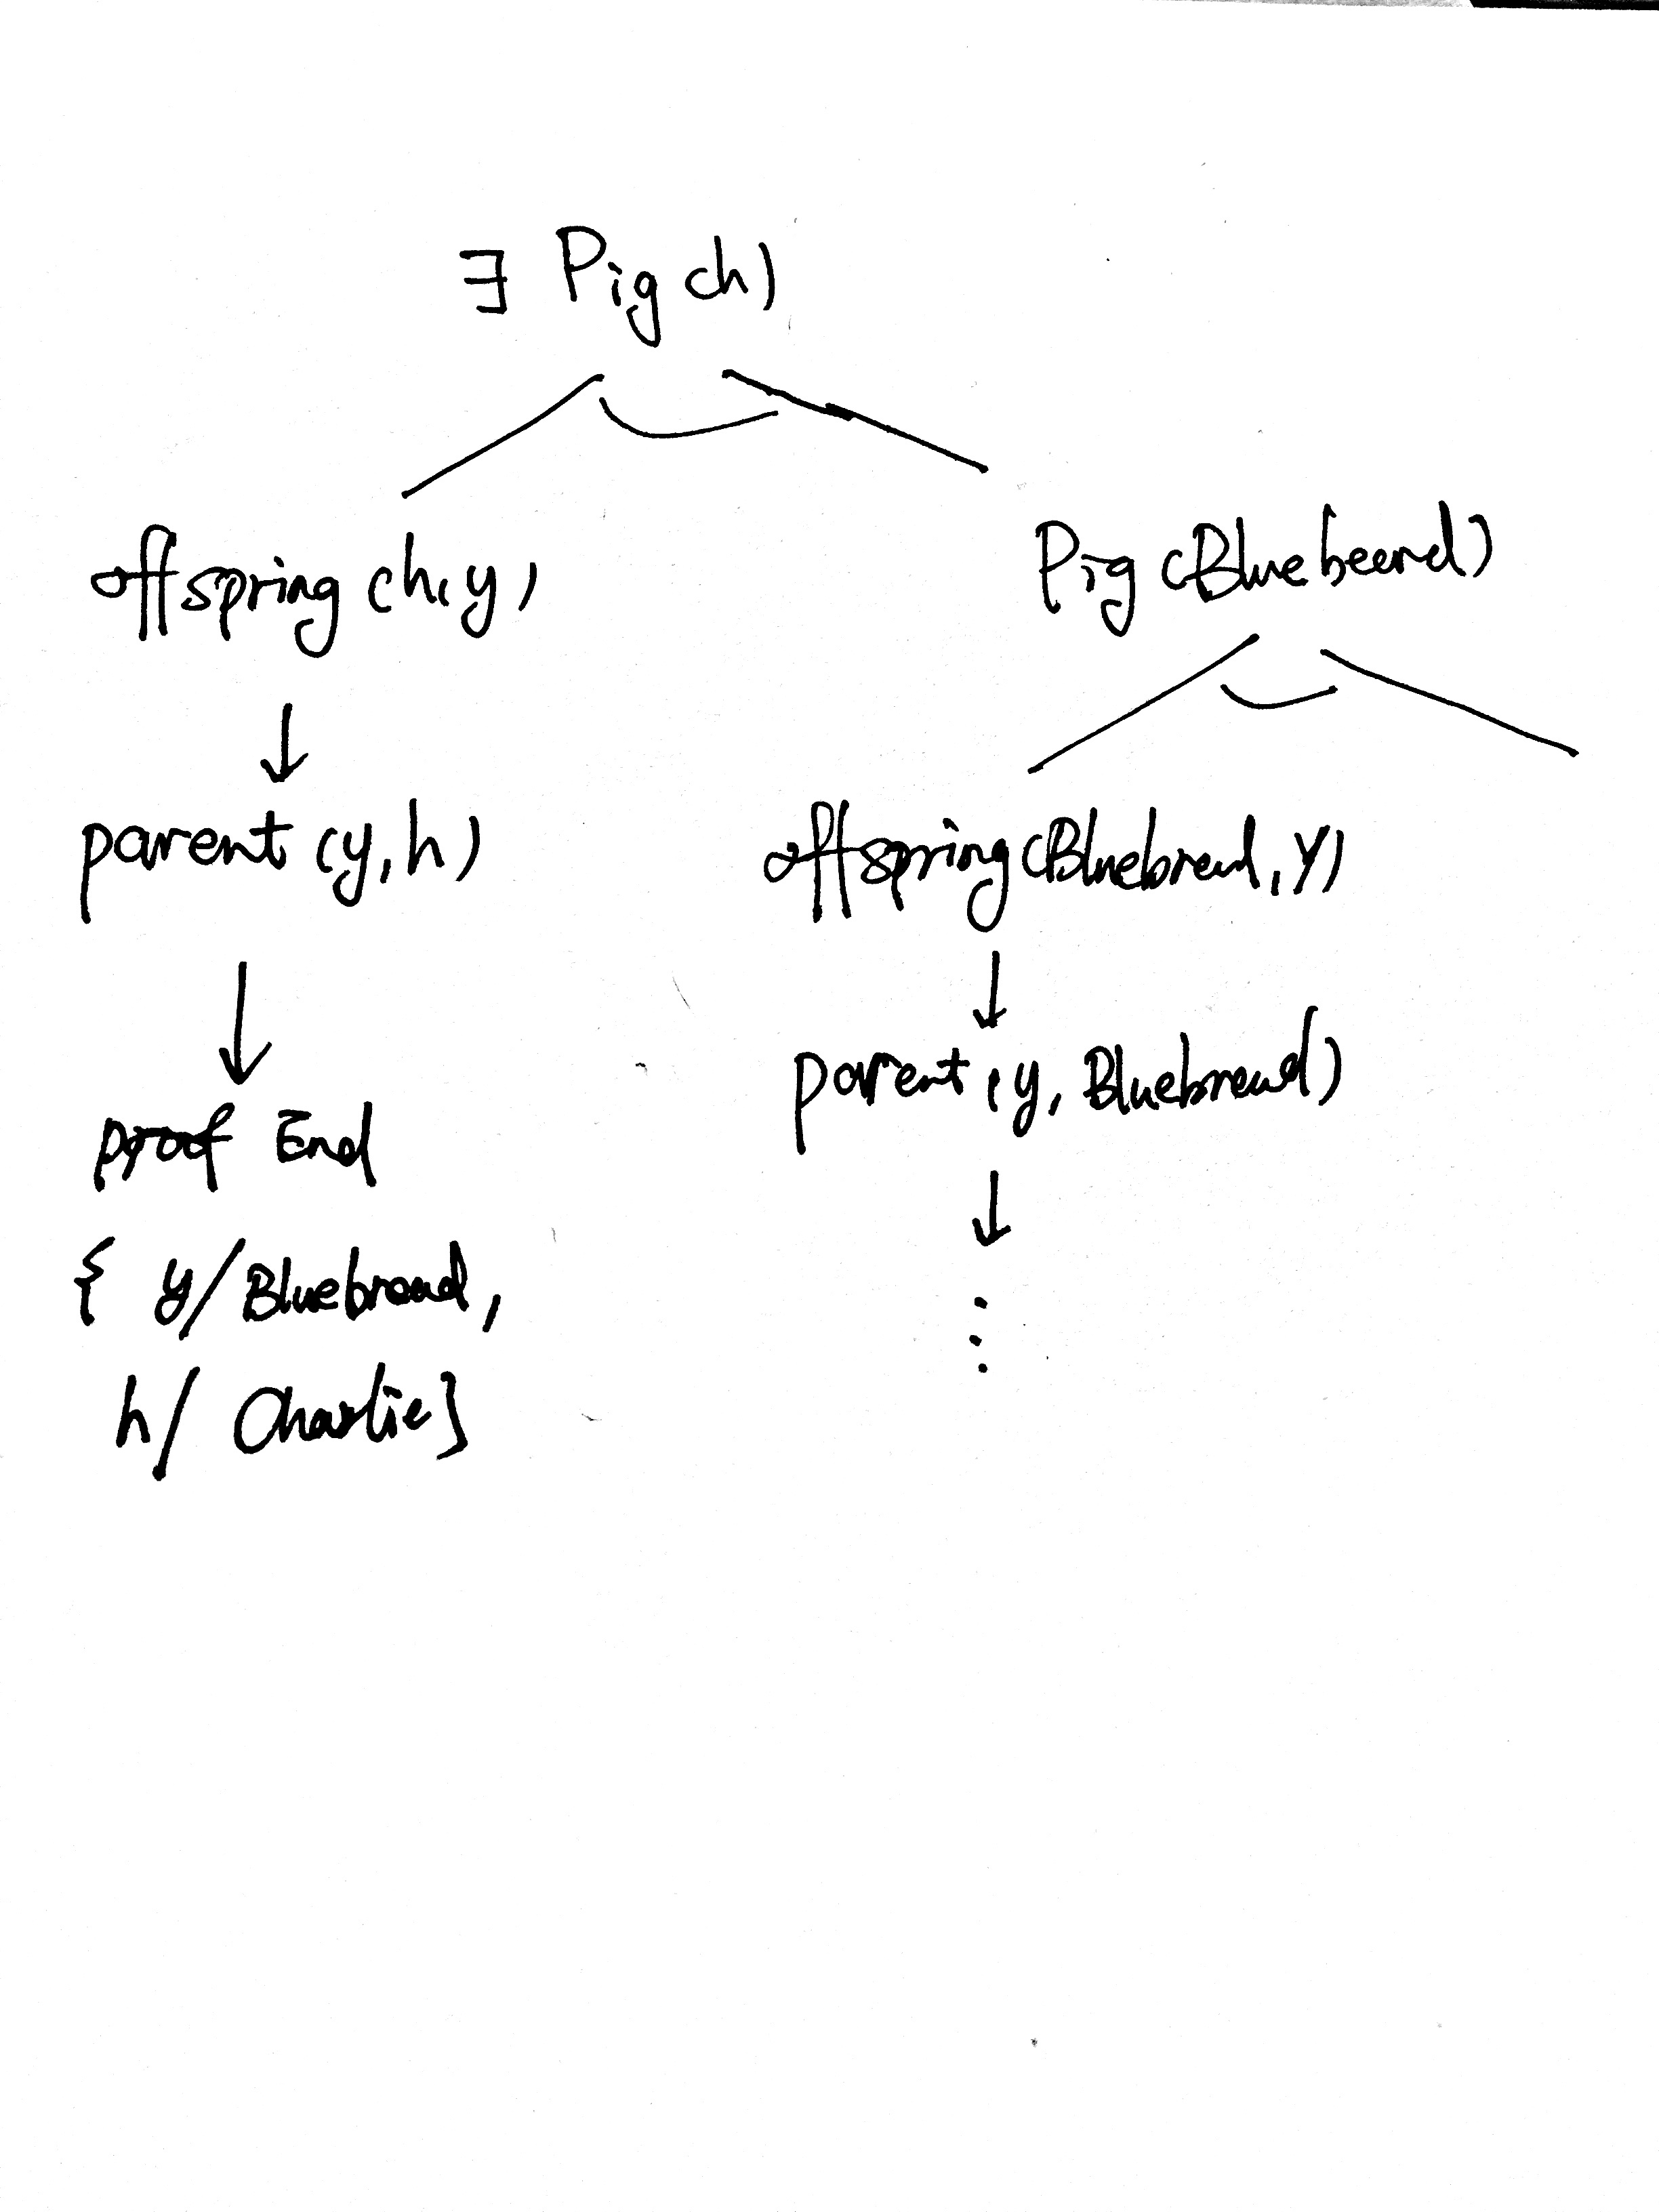
\includegraphics[width=4  in]{1.jpg}\par
\item[Problem 7]\textbf{Solution:}\par
\begin{enumerate}
	\item 
	\begin{eqnarray*}
		&&((\exists x)[P(x)] \lor (\exists x)[Q(x)])\Rightarrow (\exists y)[P(y) \lor Q(y)]\\
		&&\neg ((\exists x)[P(x)] \lor (\exists x)[Q(x)]) \lor (\exists y)[P(y) \lor Q(y)]\\
		&&((\forall x)[P(x)] \land (\forall x)[Q(x)]) \lor P(Y) \lor Q(Y)\\
		&&(\neg P(x_1)\land \neg Q(x_1)) \lor P(Y) \lor Q(Y)\\
		&&(\neg P(x_1)\lor P(Y) \lor Q(Y)) \land (\neg Q(x_1) \lor P(Y) \lor Q(Y))
	\end{eqnarray*}

	\item 
	\begin{eqnarray*}
	&&(\exists x)[P(x)] \Rightarrow (\exists z)[(\forall x)[Q(x,z)] \lor (\forall x)[R(x,y,z)]]\\
	&&\neg (\exists x)[P(x)] \lor (\exists z)[(\forall x)[Q(x,z)] \lor (\forall x)[R(x,y,z)]]\\
	&&(\forall x) [\neg P(x)] \lor (\exists z)[(\forall x)[Q(x,z)] \lor (\forall x)[R(x,y,z)]]\\
	&&\neg P(x_1) \lor [Q(x_2,Z) \lor R(x_3,y,Z)\\
	\end{eqnarray*}
	\item 
	\begin{eqnarray*}
		&& (\forall x)[P(x) \Rightarrow Q(x,y)] \Rightarrow ((\exists y)[P(y)] \land (\exists v)[Q(y,v)])\\
		&& \neg (\forall x)[\neg P(x) \lor Q(x,y)] \lor ((\exists y)[P(y)] \land (\exists v)[Q(y,v)])\\
		&& (\exists x)[ P(x) \land \neg Q(x,y)] \lor (P(Y) \land Q(y,V))\\
		&& (P(X) \land \neg Q(X,y)) \lor (P(Y) \land Q(y,V))\\
		&& (P(X) \lor P(Y)) \land (P(X) \lor Q(y,V))  \land (\neg Q(X,y) \lor P(Y)) \land (\neg Q(X,y) \lor Q(y,V))
	\end{eqnarray*}
\end{enumerate}
\item[Problem 8]\textbf{Solution:}\par
\begin{enumerate}
	\item
		\begin{eqnarray*} 
		&&(\exists x)[Blue(x)\land Push(x)] \Rightarrow (\forall y)[\neg Push(y)\Rightarrow Green(y)]\\
		&&(\forall x)[(Blue(x)\land \neg Green(x)) \lor (\neg Blue(x) \land Green(x)) ]\\
		&&(\exists x)[\neg Push(x)] \Rightarrow (\forall y)[Push(y)\Rightarrow Blue(y)]\\
		&&Push(01)\\
		&&\neg Push(02)
		\end{eqnarray*}
	\item
	\begin{eqnarray*} 
		&&\neg Blue(x_1)\lor \neg Push(x_1) \lor Push(y_1) \lor Green(y_1)\\
		&&(Blue(x_2)\lor Green(x_2)) \land (\neg Blue(x_2) \lor \neg Green(x_2))\\
		&& Push(x_3) \lor \neg Push(y_2)\lor Blue(y_2)\\
		&&Push(01)\\
		&&\neg Push(02)
	\end{eqnarray*}
	\item
	answer term $(\exists x) Green(x)$.\\
	 Negating the answer term, obtain $\neg Green(x_4)$.
	\begin{eqnarray}
		&&\neg Blue(x_1)\lor \neg Push(x_1) \lor Push(y_1) \lor Green(y_1)\\
		&&(Blue(x_2)\lor Green(x_2)) \land (\neg Blue(x_2) \lor \neg Green(x_2))\\
		&& Push(x_3) \lor \neg Push(y_2)\lor Blue(y_2)\\
		&&Push(01)\\
		&&\neg Push(02)\\
		&&\neg Green(x_4)\\
		&&Push(02) \lor \neg Push(01)\lor Blue(01) \{ 16, x_3/02, y_2/01\} \\
		&&Blue(01) \text{ (17,18,19,20)}\\
		&&\neg Blue(01)\lor \neg Push(01) \lor Push(02) \lor Green(02)\{14, x_1/01,y1/02 \} \\
		&&Green(02)\{17,18,21,22,\}\\
		&&\neg Green(02)\{19, x_4/02\}\\
		&&Empty\{23,24\}
	\end{eqnarray}
	Thus, answer has been proofed.
\end{enumerate}
\end{enumerate}
\end{document}
